\documentclass[main_estudante.tex]{subfiles}

\begin{document}

\chapter{Revisão para integrais trigonométricas}

\section{Comentários iniciais}

Esse capítulo é focado em algumas identidades trigonométricas que são fundamentais para as técnicas de integração chamadas \textbf{integrais trigonométricas} e \textbf{subsituição trigonométricas}.

Além de relembrar essas identidades, este capítulo foca em usos compatíveis com o que será feito na disciplina de Cálculo Diferencial e Integral.

Ao longo do capítulo algumas integrais envolvendo as funções trigonométricas seno, cosseno e tangente serão necessárias.

Um ponto importante em relação às identidades trigonométricas é que os estudantes vejam que todas podem ser obtidas a partir de um conjunto menor formado, essencialmente por:

$$\sin^2(x)+\cos^2(x)=1$$

$$\sin(a+b)=\sin(a)\cos(b)+\sin(b)\cos(a)$$

$$\cos(a+b)=\cos(a)\cos(b)-\sin(a)\sin(b) $$

A primeira pode ser rapidamente obtida a partir do teorema de pitágoras, mas as outras duas são mais trabalhosas para obter e precisam ser decoradas. Além de lembrar das identidades acima, é importante saber como usá-la e esperamos que a sequência de questões propostas faça esse trabalho.

\section{Quando usar}

Como este capítulo cobre tópicos relacionados a duas técnicas de integração, seus estudantes talvez tenham mais tempo para se dedicar a ele. Certifique-se de que o professor dos estudantes da sua turma esteja prestes a iniciar o tópico \textbf{integrain trigonométricas} ou tenha acabado de iniciá-lo. Esse é o momento ideal para usar este capítulo.

\section{Questões comentadas}

\begin{questao}
Considerando a função $f(x)=\sqrt{4-x^2}$, responda:
\begin{enumerate}[a)]
\item Qual é o seu domínio?
\item Quais são as raízes da função?
\item Em que ponto o seu gráfico corta o eixo $Y$?
\item Qual é a imagem da função?
\end{enumerate}
\end{questao}

\begin{questao}
Manipule algebricamente a função na forma $y=\sqrt{4-x^2}$ de modo a obter uma expressão que seja familiar. 
\begin{enumerate}[a)]
\item Que curva essa expressão representa?
\item Esboce o gŕafico da função $f(x)$.
\end{enumerate}
\end{questao}

As duas primeiras questões bastante introdutórias e tem como objetivo estabelecer bem o cenário que servirá para esete capítulo. Na verdade, o capítulo todo girará em torno da resolução (e entendimento) da integral de $f(x)$.

\begin{questao}
Vamos considerar agora a integral $\int_{-2}^{2} f(x)dx$.
\begin{enumerate}[a)]
\item Qual é o significado geométrico dessa integral?
\item Com base na resposta anterior, qual deve ser o valor da integral (sem efetuar a integração de fato)?
\end{enumerate}
\end{questao}

Ainda em aspectos introdutórios, essa questão tenta salientar uma possível conexão entre a integral pedida e funções trigonométricas.

\begin{questao}
Para que você sinta a dificuldade, tente obter um integrando mais simples usando a troca de variáveis $u=4-x^2$. Qual é a nova integral obtida?
\end{questao}

Essa questão busca convencer o estudante de que a integral pedida não pode ser resolvida através de uma simples troca de variável. Não deixe que eles gastem muito tempo com ela.

\begin{questao}
Considerando o triângulo retângulo abaixo:
\begin{enumerate}[a)]
\item Use o teorema de pitágoras para obter uma expressão para o comprimento do cateto vertical.
\item Use as relações trigonométricas acerca do ângulo $\theta$ para obter uma outra expressão para o comprimento do cateto vertical.
\item Use as relações trigonométricas acerca do ângulo $\theta$ para obter uma outra expressão para o comprimento do cateto $x$.
\end{enumerate}
\end{questao}

\begin{figure}[h]
\centering
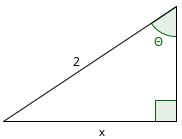
\includegraphics[width=0.25\textwidth]{./img/l2q4.png}
\end{figure}

Neste momento introduzimos um argumento geométrico para a troca de variáveis que será feita e que fundamenta a técnica de integração chamada de substituição trigonométrica.

\begin{questao}
Rescreva a integral $\int_{-2}^{2} \sqrt{4-x^2}dx$ usando a troca de variáveis $\sqrt{4-x^2}=\cos(\theta)$ (lembre-se que $x=2\sin(\theta)$).
\end{questao}

Finalmente foi realizada a troca de variáveis. Apesar de o texto salientar que o diferencial e os limites da integral devem ser ajustados, certifique-se de que os estudantes estão dando atenção a esses pontos. Se eles estiverem com muitas dificuldades nesse momento é prvável que estejam com dificuldades em integrais como um todo. Nesse caso, sugira que calculem as integrais indefinidas $\int e^{2x+3}dx$ e $\int x.\sin(x^2)dx$. Se os estudantes não conseguirem resolvê-las, eles estão com dificuldades mais básicas sobre a regra da substituição e você pode recomendar a leitura dos exemplos da seção 5.5 do livro \sugestao{Calculus}. Se eles conseguirem, provavelmente vale a pena ajudá-los passo-a-passo com a troca de variáveis desse caso especificamente.

\begin{questao}
Considerando as igualdades acima:
\begin{enumerate}[a)]
\item Qual troca de variável você utilizaria se a função a ser integrada fosse $g(x)=\sqrt{1+x^2}$?
\item Como ficaria a integral $\int \sqrt{1+x^2} dx$ quando essa troca for completada?
\end{enumerate}
\end{questao}

Essa questão foi inclusa para chamar a atenção para o impacto que o sinal do termo dentro da raiz tem sobre a escolha da troca a ser usada.

\begin{questao}
Considerando as igualdades acima:
\begin{enumerate}[a)]
\item Isole $\cos^2(\alpha)$ na primeira igualdade.
\item Use as duas igualdades para converter a expressão $\cos^3(a)$ em uma expressão em que apareça senos e cossenos, mas nenhum deles com potências maiores do que 1. Dica: $\cos^3(a) = \cos^2(a) \cdot \cos(a)$
\item Use a igualdade $\sin^2(a) + \cos^2(a)=1$ vista anteriormente e a primeira igualdade acima para obter uma expressão que transforma $\sin^2(a)$ em $\cos(2a)$.
\item Rescreva a expressão $\sin^4(a)$ como uma expressão composta por senos e cossenos com as menores potências possíveis.
\end{enumerate}
\end{questao}

Essa questão explora as igualdades frequentemente utilizadas na técnica de integração chamada de integrais trigonométricas e que é normalmente aplica a potências de senos e cossenos. Como ressaltado no texto para o aluno, as igualdades permitem a redução da potência em senos e cossenos e ambas derivam das fórmulas de $\sin(a+b)$ e $\cos(a+b)$.

O último item da questão exige o uso da identidade duas vezes consecutivas. Apesar de destoar das demais questões propostas devido à quantidade de manipulações algébricas, insista que os estudantes o resolvam por inteiro pois isso será esperado deles em MA111.

\begin{questao}
Rescreva $4\int_{-\pi/2}^{\pi/2} cos^2(\theta)d\theta$, usando as igualdades anteriores, de modo que não haja mais potências no integrando.
\end{questao}

Mais uma troca de variáveis, agora visando remover o quadrado do integrando.

\begin{questao}
Finalize essa questão calculando a integral obtida acima.
\end{questao}

Após a sequência de passos seguida nas questões anteriores, a integral final é relativamente simples e o resultado é esperado: $2\pi$. Fique atento a pequenas variações na resposta que podem advir de erros procedimentais, como a omissão de algum sinal ou de constantes multiplicando as expressões.

\section{Comentários finais}

Durante as atividades da tutoria não se preocupe em identificar e listar todos os casos em que as duas técnicas de integração em questão costumam ser sub-divididas. Isso será feito pelo professor de MA111. 

Por outro lado, é importante que os estudantes consigam lembrar das identidades trigonométricas utilizadas ao longo do capítulo. Insista na importância desse aspecto!

Após resolverem as questões propostas, sugerimos aos estudantes que leiam alguns exemplos das seções 7.2 e 7.3 do livro \sugestao{Calculus} e então partam para a lista de exercícios da disciplina.

\section{Gabarito}

\noindent\textbf{Questão 1:} a) $[-2;2]$, b) $-2$ e $2$, c) $(0;2)$, d) $[0;2]$.

\noindent\textbf{Questão 2:} a) circunferência de raio 2 e centro na origem.

\noindent\textbf{Questão 3:} a) a integral é igual à área de uma semi-circunferência de raio 2, b) $2\pi$.

\noindent\textbf{Questão 4:} $-2\int\sqrt{4u-u^2}du$

\noindent\textbf{Questão 5:} a) $\sqrt{4-x^2}$, b) $2\cos(\theta)$, c) $2\sin(\theta)$.

\noindent\textbf{Questão 6:} $4 \int_{-\pi/2}^{\pi/2} \cos^2(\theta)d\theta$.

\noindent\textbf{Questão 7:} a) $x=\tan(\alpha)$ e, portanto, $\sqrt(4+x^2)=\sec(\alpha)$, b) $\int \sec^3(\alpha)d\alpha$.

\noindent\textbf{Questão 8:} a) $\cos^2(\alpha)=\frac{\cos(2\alpha)+1}{2}$, b) $\sin^2(\alpha)=\frac{1-\cos(2\alpha)}{2}$, c) $\sin^4(\alpha)=\frac{1}{8} \cdot (3-4\cos(2\alpha)+\cos(4\alpha))$.

\end{document}
